\documentclass[a4paper,11pt,openany]{book}
\usepackage[T1]{fontenc}
\usepackage[utf8]{inputenc}
\usepackage[french]{babel}
\usepackage{lmodern} % Latin Modern font
\usepackage{pifont} % DingBats font

\usepackage
[
        a4paper,% other options: a3paper, a5paper, etc
        left=2cm,
        right=2cm,
        top=3cm,
        bottom=4cm,
        % use vmargin=2cm to make vertical margins equal to 2cm.
        % us  hmargin=3cm to make horizontal margins equal to 3cm.
        % use margin=3cm to make all margins  equal to 3cm.
]
{geometry}% layout
\usepackage{graphicx}
\usepackage{amssymb}
\usepackage{amsmath}
\usepackage{listings}
\usepackage{longtable}
\usepackage{adjustbox}
\usepackage{caption}
\captionsetup{font=small}
\usepackage{appendix}
%\usepackage{hyperref}
\renewcommand{\footnotesize}{\scriptsize}
\usepackage[pdftex,% utility for pdf format
    pagebackref=false,% pas de renvoi vers pages de citation
    hyperfootnotes=false,
    linktocpage=true,% link with page number instead of whole line
    breaklinks=true,% links possible on several lines 
    colorlinks=true,% links in color and no box
    citecolor=blue,
    hyperindex,%
    pdffitwindow,
    pdfpagemode=UseOutlines,%=None,%UseNone,
    hypertexnames=true, %false
    bookmarksopen=true]{hyperref} % hyperlinks for references
\usepackage{tikz}
\usetikzlibrary{arrows.meta, positioning, calc, shapes.geometric}
\usepackage{xcolor}
\usepackage{float}
\usepackage{tabularx}
\usepackage{booktabs}

\usepackage{color}
\usepackage{multirow}
\usepackage{subfigure}

\makeatother
\definecolor{codegreen}{rgb}{0,0.6,0}
\definecolor{airforceblue}{rgb}{0.36, 0.54, 0.66}
\definecolor{codegray}{rgb}{0.5,0.5,0.5}
\definecolor{codepurple}{rgb}{0.58,0,0.82}
\definecolor{backcolour}{rgb}{0.95,0.95,0.92}
\definecolor{primaryColor}{RGB}{44, 62, 80}
\definecolor{secondaryColor}{RGB}{231, 76, 60} 

\lstdefinestyle{mystyle}{
	backgroundcolor=\color{backcolour},   
	commentstyle=\color{airforceblue},
	keywordstyle=\color{magenta},
	numberstyle=\tiny\color{codegray},
	stringstyle=\color{codepurple},
	basicstyle=\footnotesize,
	breakatwhitespace=false,         
	breaklines=true,                 
	captionpos=b,                    
	keepspaces=true,                 
	numbers=left,                    
	numbersep=5pt,                  
	showspaces=false,                
	showstringspaces=false,
	showtabs=false,                  
	tabsize=2
}

\usepackage{adjustbox}
\usepackage{longtable}
\usepackage{multirow}
\usepackage{subfigure}
%\renewcommand\UrlFont{\color{blue}\rmfamily}

\newcommand{\ie}{\textit{i.e.,} }
\newcommand{\eg}{\textit{e.g.,} }
\newcommand{\etal}{\textit{et al.}}

% Nom du chapitre bibliographie (évite "Bibliography")
\renewcommand{\bibname}{Bibliographie}

\lstset{
  style=mystyle,
  inputencoding=utf8,
  extendedchars=true,
  literate=
    {á}{{\'a}}1 {à}{{\`a}}1 {â}{{\^a}}1 {ä}{{\"a}}1
    {Á}{{\'A}}1 {À}{{\`A}}1 {Â}{{\^A}}1 {Ä}{{\"A}}1
    {ç}{{\c{c}}}1 {Ç}{{\c{C}}}1
    {é}{{\'e}}1 {è}{{\`e}}1 {ê}{{\^e}}1 {ë}{{\"e}}1
    {É}{{\'E}}1 {È}{{\`E}}1 {Ê}{{\^E}}1 {Ë}{{\"E}}1
    {í}{{\'i}}1 {ì}{{\`i}}1 {î}{{\^i}}1 {ï}{{\"i}}1
    {Í}{{\'I}}1 {Ì}{{\`I}}1 {Î}{{\^I}}1 {Ï}{{\"I}}1
    {ó}{{\'o}}1 {ò}{{\`o}}1 {ô}{{\^o}}1 {ö}{{\"o}}1
    {Ó}{{\'O}}1 {Ò}{{\`O}}1 {Ô}{{\^O}}1 {Ö}{{\"O}}1
    {ú}{{\'u}}1 {ù}{{\`u}}1 {û}{{\^u}}1 {ü}{{\"u}}1
    {Ú}{{\'U}}1 {Ù}{{\`U}}1 {Û}{{\^U}}1 {Ü}{{\"U}}1
    {œ}{{\oe}}1 {Œ}{{\OE}}1
}

\begin{document}

\newcommand{\HRule}{\rule{\linewidth}{0.5mm}} % valeur classique
\newcommand\myfontsize{\fontsize{13pt}{14pt}\selectfont}
\newcommand\monfontsize{\fontsize{29pt}{27pt}\selectfont}

\thispagestyle{empty}

\begin{center}
\vfill

% Upper part of the page. The '~' is needed because only works if a paragraph has started.
\IfFileExists{Figures/ENSIIE01.png}{
\includegraphics[height=3cm]{Figures/ENSIIE01}~\\[.4cm]}{%
\IfFileExists{Figures/ENSIIE01.pdf}{
\includegraphics[height=3cm]{Figures/ENSIIE01}~\\[.4cm]}{%
{\large \textbf{ENSIIE}}\\[.4cm]
}}

{\large École Nationale Supérieure d'Informatique pour l'Industrie et l'Entreprise\\[1.0cm]}

% Title
%\HRule \\[0.5cm]

{\monfontsize \bfseries Rapport de stage de 2\textsuperscript{ème} année\\[0.6cm]}
{\Large \bfseries « Conception et développement d’une plateforme full-stack dédiée à l’artisanat d’art »\\[0.5cm] }

\HRule \\[1.0cm]

{\large
\emph{Étudiante} : \textbf{Manal Derghal}\\
\emph{Tuteur académique} : \textbf{Julien Forest}\\[1.5cm]

\IfFileExists{Figures/enterprise.png}{
\includegraphics[height=6cm]{Figures/enterprise}~}{%
\IfFileExists{Figures/enterprise.jpg}{
\includegraphics[height=6cm]{Figures/enterprise}~}{%
\IfFileExists{Figures/enterprise.pdf}{
\includegraphics[height=6cm]{Figures/enterprise}~}{}
}}
\hspace{1cm} 
    
\emph{Entreprise} : \textbf{RUHENNA} -- Rue Edmond Boris, 78130 Les Mureaux\\[0.5cm]
\emph{Maître de stage} : \textbf{Sumeyra Solak}\\[1.5cm]

\emph{Dates} : \textbf{Du 19 janvier au 13 mars 2026}\\
} % Fin \large
        
\end{center}

\newpage
\thispagestyle{empty}
\pagenumbering{roman}  % <-- Start Roman numbering

\chapter*{Résumé}
\addcontentsline{toc}{chapter}{Résumé}
Ce rapport présente le travail réalisé au sein de l’entreprise \textbf{RUHENNA}, une activité artisanale portée par \textbf{Sumeyra Solak}, dans le cadre d’un stage de 2\textsuperscript{ème} année. L’objectif du projet était de concevoir et développer une plateforme web \textit{full-stack} permettant de renforcer l’image de marque, de valoriser les créations autour de l’art du henné et de simplifier la gestion opérationnelle (catalogue de produits, prise de rendez-vous, blog et formulaire de contact), tout en offrant un \textbf{panneau d’administration} pour centraliser l’édition du contenu et le suivi des demandes.

La solution s’appuie sur une architecture moderne basée sur \textbf{React} et \textbf{Next.js} (App Router), \textbf{Prisma} comme ORM, et une base de données \textbf{PostgreSQL} hébergée sur \textbf{Neon} pour faciliter le déploiement sur \textbf{Vercel}. La gestion des médias s’appuie sur \textbf{Cloudinary} afin d’optimiser le stockage et la diffusion d’images. Une attention particulière a été portée à l’expérience utilisateur (interfaces publiques et administration), à la structuration des données (modèle relationnel, contraintes d’intégrité) et à la maintenabilité (typage TypeScript, validation des entrées, séparation des responsabilités).

Au-delà des aspects techniques, ce stage a constitué une montée en compétences progressive sur React/Next.js et Prisma, depuis un niveau initial limité, à travers un apprentissage guidé par la documentation et des ressources en ligne, puis par la confrontation à des problèmes réels (routage, interaction front/back, disponibilité de créneaux, gestion d’images, déploiement).


\section*{Mots-clés}
\noindent \textbf{Mots-clés :} Next.js, React, Prisma, PostgreSQL, réservation, back-office, Cloudinary, Zod, TipTap, @dnd-kit.

\newpage
\thispagestyle{empty}

\tableofcontents

\newpage
\pagenumbering{arabic} % <-- Switch to Arabic numbering

\chapter{Introduction : environnement de travail et stage}\label{ch:Introduction}
\section{Présentation de l’environnement}
Ce stage de 2\textsuperscript{ème} année a été réalisé au sein de \textbf{RUHENNA}, une activité artisanale portée par \textbf{Sumeyra Solak} et centrée sur l’art du henné (prestations pour événements et produits associés). La structure étant de petite taille, l’enjeu principal était de livrer une solution \textbf{simple à utiliser} et \textbf{administrable} au quotidien.

\section{Sujet et objectifs du stage}
Le sujet du stage était de participer à la conception et au développement d’une plateforme web \textit{full-stack} permettant :
\begin{itemize}
    \item de valoriser la marque et les réalisations (galerie, blog) ;
    \item de rendre l’offre lisible (catalogue) ;
    \item de structurer les demandes (contact et réservation) ;
    \item de permettre une gestion autonome via un espace d’administration.
\end{itemize}

\section{Outils et moyens utilisés}
Le projet s’appuie sur une stack web courante : \textbf{React/Next.js} (App Router), \textbf{Prisma} et \textbf{PostgreSQL} (hébergée sur \textbf{Neon}), \textbf{Tailwind CSS}, \textbf{Cloudinary} pour les images, et un déploiement sur \textbf{Vercel}.

\section{Annonce du plan}
Le rapport présente d’abord le contexte et les choix (contraintes, outils, méthode, alternatives), puis détaille la solution mise en place, les contributions et les résultats observables (exemples de parcours, gestion admin, mise en production). Il se termine par une synthèse et des perspectives, avec des annexes techniques.


\chapter{Contexte et préliminaires}\label{ch:background}
\section{Environnement}
\subsection{Entreprise et activité}
\textbf{RUHENNA} est une activité artisanale portée par \textbf{Sumeyra Solak}. Elle propose des prestations au henné (notamment pour des événements) et des produits associés (cônes, accessoires, kits). Le henné est une teinture d’origine végétale (\textit{Lawsonia inermis}) qui permet de réaliser des motifs temporaires sur la peau, avec une dimension culturelle importante lors de certaines célébrations.

\subsection{Organisation et contraintes}
La structure ne disposant pas d’équipe informatique, les échanges ont été directs : Sumeyra porte la vision métier (offre, contenus, règles de réservation) et le stage vise à livrer un outil administrable. Le besoin a été identifié de manière concrète à la suite d’échanges initiés dans un contexte réel (Sumeyra a réalisé le henné lors de mon mariage), puis formalisé en fonctionnalités et règles simples.

\section{Problématique : contexte et objectifs}
Avant la plateforme, la présence en ligne et la gestion des demandes pouvaient être dispersées (réseaux sociaux, messages, échanges manuels). L’objectif a donc été de concevoir un site qui valorise l’activité (galerie, blog, catalogue) tout en structurant la prise de contact et la réservation, avec un back-office permettant une mise à jour autonome.

\section{Spécifications du stage (cahier des charges)}

\subsection{Exigences fonctionnelles}
Le cahier des charges fonctionnel a été construit à partir des besoins concrets de l’activité :
\begin{itemize}
    \item \textbf{Catalogue (boutique)} : afficher les produits sous forme de \textit{catalogue}, avec une page détail par produit.
    \item \textbf{Catégories} : proposer des catégories ordonnées afin de guider la navigation.
    \item \textbf{Galerie} : exposer des réalisations, avec possibilité de mise en avant.
    \item \textbf{Bannière (hero)} : gérer un carrousel d’images sur la page d’accueil.
    \item \textbf{Réservation} : permettre la sélection d’un service, d’une date et d’un créneau disponible, puis l’envoi d’une demande.
    \item \textbf{Contact} : formulaire structuré, stockage du message en base, consultation côté admin.
    \item \textbf{Blog} : création d’articles, publication/dépublication, lecture publique.
    \item \textbf{Administration} : CRUD complet des entités (produits, services, images, articles, messages, rendez-vous).
\end{itemize}

\subsection{Exigences non-fonctionnelles}
\begin{itemize}
    \item \textbf{Maintenabilité} : code lisible, typé, organisé, et facilement extensible.
    \item \textbf{Performance et UX} : mise en cache implicite, chargements fluides, formulaires guidés.
    \item \textbf{SEO} : pages indexables, métadonnées, données structurées (LocalBusiness).
    \item \textbf{Sécurité} : protection de l’admin, validation des entrées, en-têtes de sécurité.
    \item \textbf{Gestion des médias} : upload sécurisé, optimisation des images.
\end{itemize}

\section{Méthodologie et outils mobilisés}

\subsection{Approche de réalisation}
L’activité RUHENNA étant de petite taille, il n’existait pas de méthodologie projet formalisée (Scrum complet, etc.). Le travail a néanmoins été structuré par une logique itérative :
\begin{enumerate}
    \item \textbf{Cadrage} : clarification des fonctionnalités prioritaires (vitrine, galerie, réservation, admin).
    \item \textbf{Modélisation} : construction du schéma de données (Prisma/PostgreSQL).
    \item \textbf{Implémentation verticale} : livraison d’une fonctionnalité complète (UI + API + DB), puis stabilisation.
    \item \textbf{Validation} : tests manuels et retours d’usage (cohérence des formulaires, lisibilité admin).
\end{enumerate}

\subsection{Montée en compétences}
Un point important du stage est le niveau initial : il y avait \textbf{peu de maîtrise préalable} de React/Next.js et de Prisma. L’apprentissage s’est appuyé sur :
\begin{itemize}
    \item la documentation officielle;
    \item des tutoriels en ligne;
    \item l’expérimentation directe.
\end{itemize}
Cette approche a été déterminante : l’apprentissage a progressé au rythme des problèmes réels.

\subsection{Outils et briques techniques du projet}
Les principaux outils observés dans le code sont :
\begin{itemize}
    \item \textbf{Next.js / React} pour l’interface et le routage \textit{App Router} ;
    \item \textbf{TypeScript} pour le typage et la fiabilité ;
    \item \textbf{Prisma} comme ORM ; \textbf{PostgreSQL} comme SGBD ;
    \item \textbf{Neon} pour héberger PostgreSQL de façon compatible avec le déploiement sur \textbf{Vercel} ;
    \item \textbf{Tailwind CSS} pour le style et la cohérence graphique ;
    \item \textbf{Cloudinary} pour le stockage d’images ;
    \item \textbf{Zod} pour la validation des entrées côté API ;
    \item \textbf{TipTap} pour l’édition des articles ;
    \item \textbf{@dnd-kit} pour le glisser-déposer.
\end{itemize}

\section{Choix technologiques : justification et alternatives}

\subsection{Pourquoi React et Next.js ?}
Le choix de React s’explique par la nécessité de construire deux expériences riches :
(i) un front public (galerie, boutique, blog, réservation), et (ii) un back-office interactif (formulaires, modales, tri, filtres).
Next.js a été retenu pour :
\begin{itemize}
    \item son \textbf{routage par convention} (\texttt{src/app/...}) ;
    \item ses \textbf{Route Handlers} permettant d’intégrer l’API sans serveur séparé ;
    \item le rendu hybride (Server Components / Client Components) utile pour la performance et le SEO ;
    \item l’intégration naturelle avec Vercel pour le déploiement.
\end{itemize}
Ces choix se fondent notamment sur la documentation officielle Next.js \cite{nextjsDocs}.

\subsection{Pourquoi Prisma et PostgreSQL ?}
PostgreSQL apporte un modèle relationnel robuste pour des entités structurées (produits, rendez-vous, disponibilités, messages, articles). Prisma complète cet avantage en fournissant :
\begin{itemize}
    \item un \textbf{schéma unique} (\texttt{schema.prisma}) ;
    \item des \textbf{types TypeScript} générés ;
    \item des migrations et une couche d’accès cohérente, limitant les erreurs de requêtes.
\end{itemize}
Cette approche correspond aux bonnes pratiques décrites par Prisma \cite{prismaDocs} : décrire le modèle de données dans un schéma central, versionner les évolutions via des migrations, puis utiliser le client généré (typé) pour effectuer des opérations CRUD de manière cohérente avec le schéma.

\subsection{Comparatif : autres technologies possibles (front, back, base de données)}
Afin de justifier le choix final, un comparatif synthétique d’alternatives réalistes est proposé. L’objectif n’est pas de « prouver » qu’une technologie est meilleure qu’une autre, mais d’expliquer un choix orienté \textbf{simplicité} : RUHENNA est un \textbf{petit site} (peu de données, pas de volumétrie massive) et la priorité était de livrer une solution stable et facile à maintenir.

\renewcommand{\arraystretch}{1.2}
\setlength{\tabcolsep}{6pt}
\begin{table}[H]
    \centering
    \small
    \caption{Comparatif d’alternatives (Front / Back / Base de données) — sources : documentations officielles \cite{reactDocs,nextjsDocs,vercelDocs,prismaDocs,neonDocs}.}
    \label{tab:tech_comparison}
  % --- À mettre dans ton préambule si ce n'est pas déjà fait ---
% \usepackage{array}
% \usepackage{tabularx}
% \usepackage{booktabs}
% \usepackage{multirow}

\begin{tabularx}{\textwidth}{@{} >{\raggedright\arraybackslash}p{3.0cm} >{\raggedright\arraybackslash}p{4.0cm} X >{\raggedright\arraybackslash}p{4.0cm} @{}}
    \toprule
    \textbf{Couche} & \textbf{Option} & \textbf{Avantages} & \textbf{Limites} \\
    \midrule
    \multirow{8}{*}{\textbf{Frontend}} 
        & Next.~js (React) & Bon SEO (SSR/SSG), routing par dossiers, un seul projet pour pages + API. & Courbe d’apprentissage (Server/Client), conventions spécifiques. \\
        \cmidrule{2-4}
        & Nuxt (Vue) & SSR/SSG intégrés, approche cohérente, Vue plus simple par certains profils. & Stack différente ; moins alignée avec l’écosystème React. \\
        \cmidrule{2-4}
        & Angular & Cadre complet, architecture imposée. & Plus lourd pour un petit site ; complexité initiale élevée. \\
    \midrule
    \multirow{8}{*}{\textbf{Backend}} 
        & Route Handlers Next.~js & API intégrée, un seul dépôt, mise en production simple. & À structurer proprement si le projet grossit (services, tests). \\
        \cmidrule{2-4}
        & Express / NestJS & Séparation claire, patterns backend avancés, tests faciles. & Infrastructure en plus, coût de maintenance plus élevé. \\
        \cmidrule{2-4}
        & Django / FastAPI & Productivité Python, écosystème riche. & Double stack (Python + JS), intégration front plus lourde. \\
    \midrule
    \multirow{8}{*}{\textbf{Base de données}} 
        & PostgreSQL & Contraintes, transactions, relations, robustesse. & Modèle relationnel à concevoir correctement. \\
        \cmidrule{2-4}
        & MySQL & Mature, performant, populaire. & Moins de fonctionnalités avancées, choix moins naturel selon l'hôte. \\
        \cmidrule{2-4}
        & MongoDB (NoSQL) & Flexibilité totale du schéma. & Moins adapté aux contraintes fortes (RDV, règles métier strictes). \\
    \bottomrule
\end{tabularx}
\end{table}
\renewcommand{\arraystretch}{1.0}

\section{Schémas pédagogiques : TypeScript et Prisma}

\subsection{Comprendre TypeScript : typage statique et compilation}
TypeScript apporte une vérification de types avant l’exécution. Les types sont \textbf{effacés} après compilation : l’exécution se fait en JavaScript.
Le schéma de la Figure~\ref{fig:ts_pipeline} est inspiré du fonctionnement décrit dans la documentation TypeScript \cite{typescriptDocs}.

\begin{figure}[H]
    \centering
    \begin{tikzpicture}[
        node distance=10mm,
        box/.style={draw, rounded corners, align=center, inner sep=7pt, text width=0.26\textwidth},
        arrow/.style={-{Stealth[length=2.2mm]}, thick}
    ]
    \node[box] (ts) {\textbf{Code TypeScript}\\\small (\texttt{.ts}, \texttt{.tsx})};
    \node[box, right=of ts] (tsc) {\textbf{Compilateur} \texttt{tsc}\\\small vérifie les types};
    \node[box, right=of tsc] (js) {\textbf{JavaScript}\\\small (\texttt{.js}) exécuté};
    \draw[arrow] (ts) -- node[above]{\small compilation} (tsc);
    \draw[arrow] (tsc) -- node[above]{\small émission} (js);
    \end{tikzpicture}
    \caption{Schéma simplifié du fonctionnement TypeScript : vérification à la compilation, exécution en JavaScript.}
    \label{fig:ts_pipeline}
\end{figure}

\subsection{Comprendre Prisma : schéma, migrations et client}
Prisma s’articule autour d’un schéma déclaratif (\texttt{schema.prisma}) décrivant les modèles. À partir de ce schéma, on obtient :
\begin{itemize}
    \item des \textbf{migrations} qui matérialisent les tables/contraintes dans PostgreSQL ;
    \item un \textbf{client Prisma} typé, utilisé dans le code Next.js.
\end{itemize}
La Figure~\ref{fig:prisma_cycle} synthétise le cycle recommandé dans la documentation Prisma \cite{prismaDocs}.

\begin{figure}[H]
    \centering
    \begin{tikzpicture}[
        node distance=10mm,
        box/.style={draw, rounded corners, align=center, inner sep=7pt, text width=0.28\textwidth},
        arrow/.style={-{Stealth[length=2.2mm]}, thick}
    ]
    \node[box] (schema) {\textbf{Schéma Prisma}\\\small \texttt{prisma/schema.prisma}};
    \node[box, right=of schema] (migrate) {\textbf{Migrations}\\\small \texttt{prisma migrate}};
    \node[box, right=of migrate] (db) {\textbf{PostgreSQL}\\\small tables, index, contraintes};
    \node[box, below=of migrate] (client) {\textbf{Prisma Client}\\\small \texttt{prisma generate}};
    \node[box, right=of client] (app) {\textbf{Application Next.js}\\\small requêtes typées};
    \draw[arrow] (schema) -- (migrate);
    \draw[arrow] (migrate) -- (db);
    \draw[arrow] (schema) -- (client);
    \draw[arrow] (client) -- (app);
    \draw[arrow] (app) -- node[above]{\small SQL via driver} (db);
    \end{tikzpicture}
    \caption{Cycle Prisma : du schéma aux migrations et au client typé.}
    \label{fig:prisma_cycle}
\end{figure}

\section{Architecture logicielle à étendre}
Le projet a été développé \textbf{from scratch} : il n’existait pas d’architecture applicative préalable au stage. En revanche, le choix de Next.js impose une architecture par conventions (dossier \texttt{app/}, layouts, routes API) qui sert de cadre structurel et garantit une cohérence globale. Le chapitre~\ref{ch:solution} détaillera cette architecture concrète à travers la structure du dépôt et les principales routes/pages.


\chapter{Solution implémentée et contributions}\label{ch:solution}
\section{Étude des solutions potentielles (avant choix final)}
Avant de stabiliser la solution, plusieurs options ont été évaluées, en cohérence avec les contraintes du projet : rapidité de développement, possibilité d’évolution (vers e-commerce), simplicité de maintenance et autonomie de l’artisane.

\subsection{Option 1 : site vitrine statique (CMS ou générateur)}
Une première approche consistait à produire un site principalement statique (WordPress, Webflow, ou générateur statique). Cette option présente des avantages (mise en ligne rapide, administration “contenu”), mais atteint rapidement ses limites dès qu’on introduit :
\begin{itemize}
    \item des règles métier (créneaux de rendez-vous, disponibilité par service) ;
    \item un back-office sur mesure (tri d’images, gestion des statuts) ;
    \item une base de données relationnelle cohérente.
\end{itemize}
Elle a donc été jugée insuffisante pour un besoin évolutif.

\subsection{Option 2 : architecture séparée Front + Back}
Une seconde approche envisageait un front (React) et un back séparé (Express/NestJS ou Django/FastAPI). Cette option est robuste, mais elle augmente le coût d’infrastructure et la charge de maintenance (deux projets, deux déploiements, plus de configuration). Pour RUHENNA, une solution monolithique Next.js est apparue plus adaptée.

\subsection{Option retenue : Next.js full-stack + Prisma + PostgreSQL}
La solution finale combine l’interface (front public et back-office) et l’API dans une seule application Next.js, avec Prisma pour le modèle de données et PostgreSQL (Neon) pour le stockage, afin d’obtenir une base saine et une mise en production simple sur Vercel.

\section{Solution implémentée : architecture et composants}

\subsection{Vue d’ensemble technique}
La plateforme est structurée autour de quatre blocs :
\begin{itemize}
    \item \textbf{Front public} : pages accessibles aux visiteurs (vitrine, galerie, blog, boutique, réservation, contact) ;
    \item \textbf{Back-office} : pages \texttt{/admin} pour gérer le contenu et les demandes ;
    \item \textbf{API} : endpoints REST via les Route Handlers Next.js (\texttt{/api/...}) ;
    \item \textbf{Données et médias} : PostgreSQL (Neon) via Prisma, et Cloudinary pour les images.
\end{itemize}

\begin{figure}[H]
    \centering
    \begin{tikzpicture}[
        node distance=10mm,
        box/.style={draw, rounded corners, align=center, inner sep=7pt, text width=0.30\textwidth},
        arrow/.style={-{Stealth[length=2.2mm]}, thick}
    ]
    \node[box] (public) {\textbf{Navigateur (public)}\\\small Pages \texttt{src/app/(main)}\\\small \texttt{/boutique}, \texttt{/galerie}, \texttt{/reservation}, ...};
    \node[box, right=of public] (api) {\textbf{API Next.js}\\\small \texttt{src/app/api/*/route.ts}\\\small validation, règles métier};
    \node[box, right=of api] (db) {\textbf{PostgreSQL (Neon)}\\\small Prisma Client\\\small données persistées};
    \node[box, below=of public] (admin) {\textbf{Navigateur (admin)}\\\small Pages \texttt{src/app/admin}\\\small gestion CRUD + tri};
    \node[box, below=of api] (cloud) {\textbf{Cloudinary}\\\small stockage et CDN images\\\small upload via \texttt{/api/upload}};
    \draw[arrow] (public) -- (api);
    \draw[arrow] (admin) -- (api);
    \draw[arrow] (api) -- (db);
    \draw[arrow] (api) -- (cloud);
    \end{tikzpicture}
    \caption{Architecture applicative : Next.js centralise UI et API, Prisma relie l’application à PostgreSQL, Cloudinary gère les médias.}
    \label{fig:architecture_tikz}
\end{figure}

\subsection{Structure du dépôt et conventions Next.js}
Le code suit l’architecture par conventions de Next.js (App Router). Les dossiers principaux sont :
\begin{itemize}
    \item \texttt{src/app/} : pages, layouts, et endpoints API ;
    \item \texttt{src/components/} : composants UI réutilisables (header/footer, éditeur, uploaders, etc.) ;
    \item \texttt{src/lib/} : accès DB, validation, configuration Cloudinary, utilitaires ;
    \item \texttt{prisma/} : schéma Prisma, migrations, seed et ERD.
\end{itemize}

\subsection{Routage : pages publiques, administration et API}
Trois familles de routes coexistent :
\begin{enumerate}
    \item \textbf{Routes publiques} : \texttt{src/app/(main)/...} (ex. \texttt{/boutique}, \texttt{/blog}).
    \item \textbf{Routes admin} : \texttt{src/app/admin/...} (ex. \texttt{/admin/produits}, \texttt{/admin/blog}).
    \item \textbf{Routes API} : \texttt{src/app/api/.../route.ts} (ex. \texttt{/api/contact}, \texttt{/api/rendez-vous}).
\end{enumerate}

\section{Base de données : schéma, entités, relations}

\subsection{Rôle de Prisma (ORM)}
Prisma agit comme une couche intermédiaire entre l’application et PostgreSQL. Les modèles sont définis dans \texttt{prisma/schema.prisma} et Prisma génère un client typé, utilisé dans les pages serveur et les routes API.

\subsection{ERD (diagramme entité-association)}
Le diagramme ERD a été généré à partir du schéma Prisma. Il permet d’illustrer les principales entités (\textit{produits, catégories, services, rendez-vous, blog, messages, images}) et les liens entre elles.

\begin{figure}[H]
    \centering
    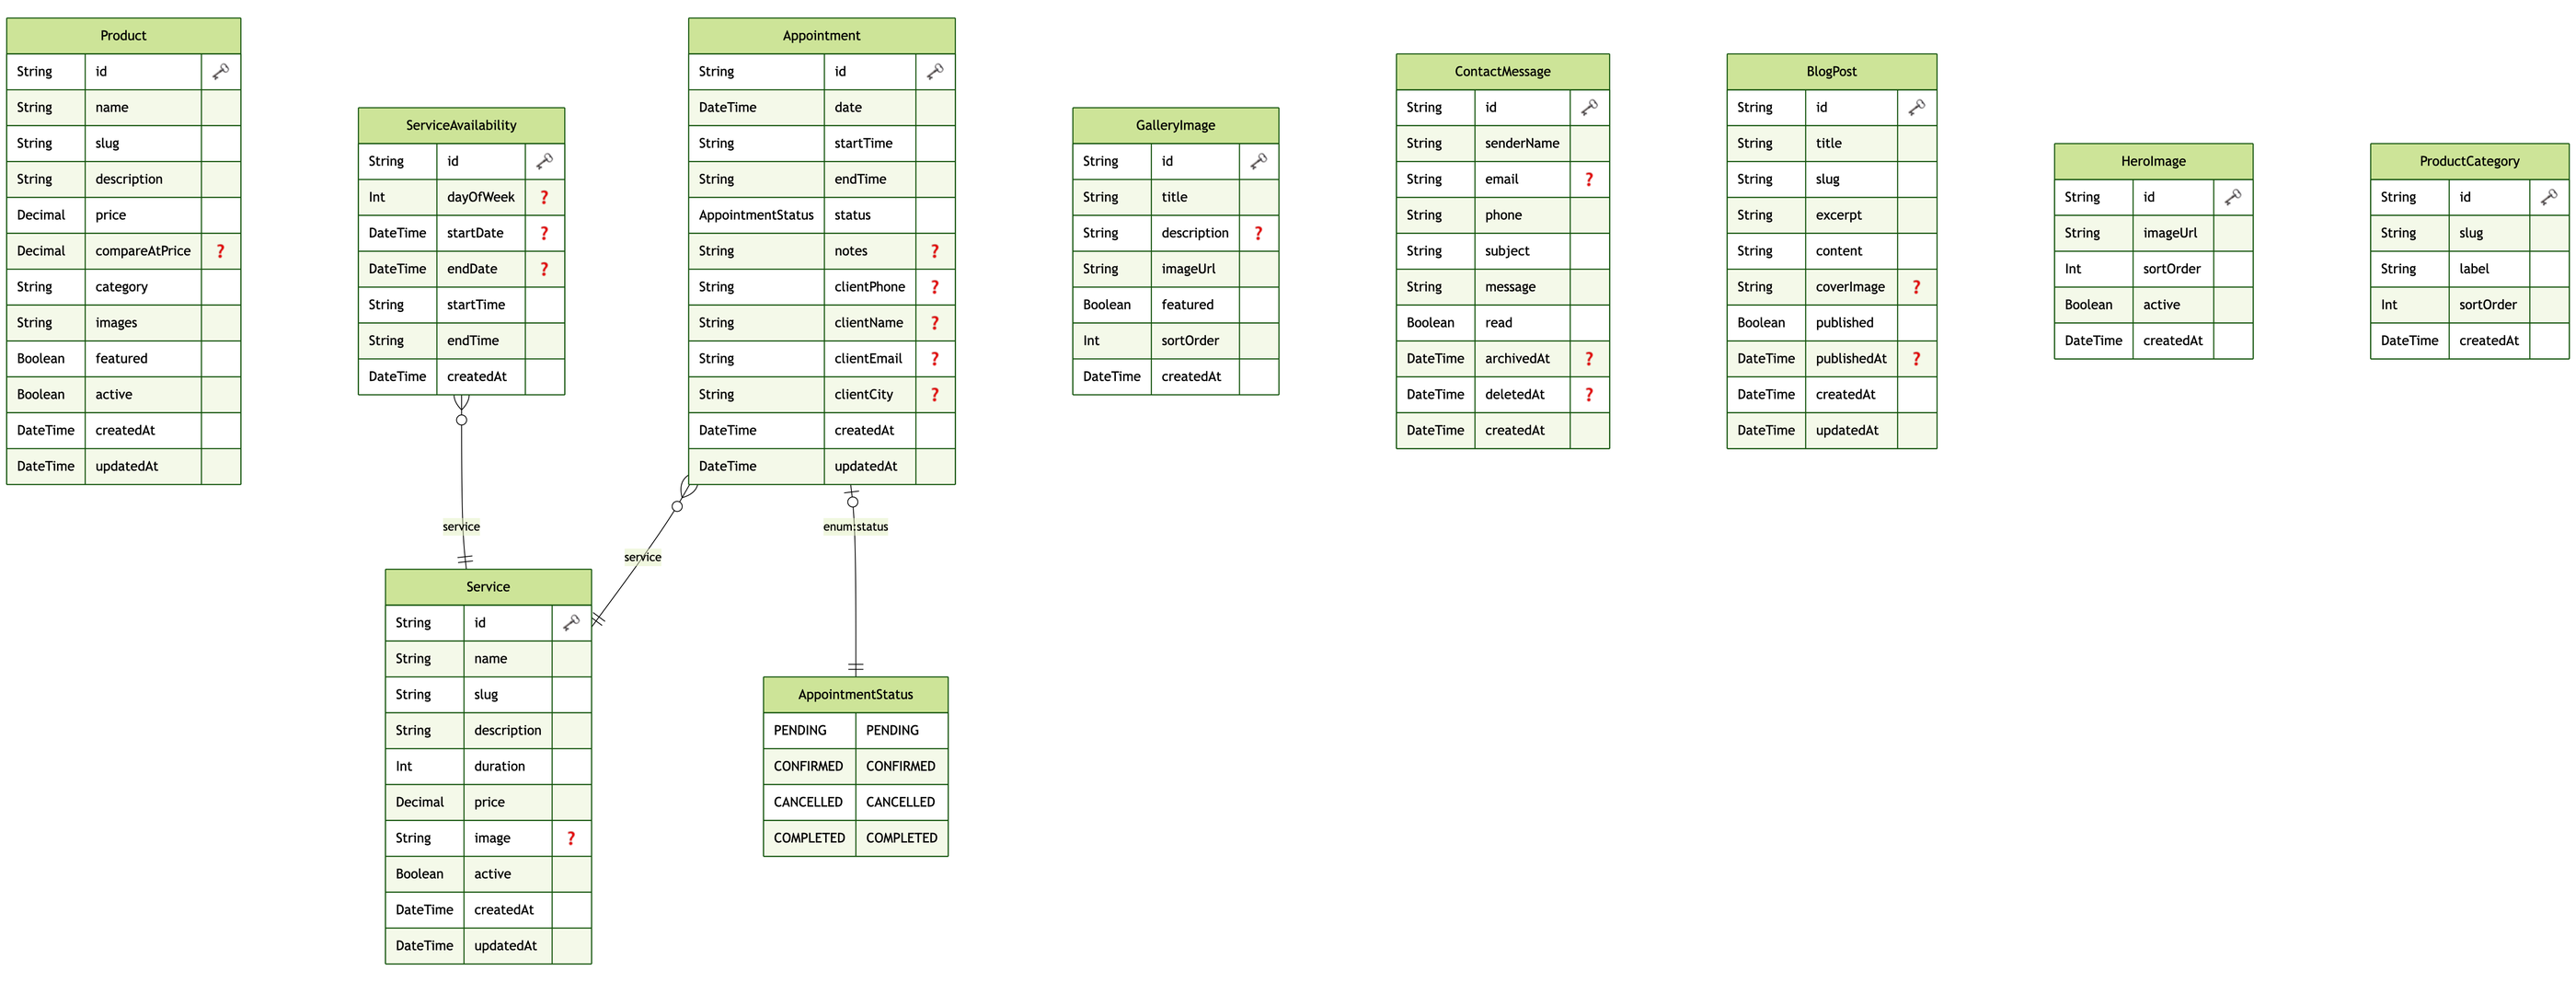
\includegraphics[width=\textwidth]{Figures/ERD.png}
    \caption{ERD de la base de données RUHENNA (généré depuis \texttt{prisma/schema.prisma}).}
    \label{fig:erd}
\end{figure}

\subsection{Modèle de données}
Le modèle de données s’organise autour d’entités qui correspondent directement aux besoins du site (catalogue, réservation, contenu, médias, messages) :
\begin{itemize}
    \item \textbf{Produits} (\texttt{Product}) : nom, description, prix, catégorie, liste d’URLs d’images (Cloudinary), statut actif/mis en avant.
    \item \textbf{Catégories} (\texttt{ProductCategory}) : liste ordonnée (champ \texttt{sortOrder}) pour maîtriser l’affichage de la boutique.
    \item \textbf{Services} (\texttt{Service}) : durée et prix, associés à des règles de disponibilité (\texttt{ServiceAvailability}).
    \item \textbf{Rendez-vous} (\texttt{Appointment}) : date, heure de début/fin, statut (en attente, confirmé, annulé, terminé).
    \item \textbf{Blog} (\texttt{BlogPost}) : titre, slug, extrait, contenu HTML, image de couverture, publication.
    \item \textbf{Messages} (\texttt{ContactMessage}) : informations du demandeur et contenu, avec gestion “lu / archivé / supprimé”.
    \item \textbf{Médias} : images de galerie et de bannière (\texttt{GalleryImage}, \texttt{HeroImage}) avec ordre d’affichage.
\end{itemize}

Pour éviter deux rendez-vous au même horaire, une contrainte d’unicité impose qu’à une date donnée, un même \texttt{startTime} ne puisse pas être réservé deux fois. Lors de la création d’un rendez-vous, l’application vérifie aussi l’absence de \textbf{chevauchement} horaire avec les rendez-vous déjà enregistrés.

\section{Fonctionnalités du front public}

\subsection{Page d’accueil et identité de marque}
La page d’accueil combine :
\begin{itemize}
    \item un \textbf{hero} avec carrousel d’images (\texttt{HeroImage}) ;
    \item une mise en avant des réalisations (\texttt{GalleryImage.featured}) ;
    \item des appels à action (galerie et réservation).
\end{itemize}
Le choix d’une page d’accueil dynamique permet de publier rapidement de nouvelles réalisations, sans redeployer manuellement des assets.

\subsection{Catalogue (boutique) : logique de lecture}
La boutique est conçue comme un \textbf{catalogue} : les produits sont consultables, filtrables par catégories, et la prise de commande passe par le contact (pas de paiement intégré à ce stade). Cette approche correspond à une phase où l’offre évolue et où l’artisane souhaite conserver un lien direct avec la clientèle.

\subsection{Galerie : consultation}
La galerie propose une grille responsive afin de mettre en valeur les réalisations, sans ajouter de complexité inutile dans le parcours utilisateur.

\subsection{Blog : contenu riche et SEO}
Les articles sont stockés en base (table \texttt{BlogPost}) et publiés/dépubliés via l’administration.

\section{Système de réservation : calcul de créneaux et création d’un rendez-vous}

\subsection{Parcours utilisateur (5 étapes)}
Le formulaire de réservation est conçu en plusieurs étapes (service, date, horaire, informations, récapitulatif) afin de réduire les erreurs et de guider la saisie.

\subsection{Calcul des créneaux disponibles (API)}
L’endpoint \texttt{/api/rendez-vous/slots} calcule les créneaux à partir :
\begin{itemize}
    \item de la durée du service ;
    \item des règles \texttt{ServiceAvailability} ;
    \item des rendez-vous existants non annulés (détection de chevauchement).
\end{itemize}

\subsection{Création d’une demande de rendez-vous}
Une fois un créneau choisi, \texttt{/api/rendez-vous} crée un enregistrement \texttt{Appointment} en statut \texttt{PENDING}. L’API vérifie :
\begin{itemize}
    \item la validité du payload (\textbf{Zod}) ;
    \item l’existence du service ;
    \item la non-disponibilité du créneau (conflit).
\end{itemize}

Le navigateur envoie un JSON minimal à l’API, avec notamment :
\begin{itemize}
    \item \texttt{serviceId} : \textit{"ck..."}
    \item \texttt{date} : \textit{"AAAA-MM-JJ"}
    \item \texttt{startTime} : \textit{"11:00"}
    \item \texttt{name/email/phone/city} : informations de contact
\end{itemize}
Si tout est valide, l’API crée un rendez-vous \textbf{en attente} et renvoie un identifiant de suivi. Si le créneau est pris entre-temps, elle renvoie un message “créneau indisponible”.

\section{Formulaire de contact : validation et stockage}

\subsection{API de contact}
La route \texttt{/api/contact} illustre l’utilisation de Zod pour valider l’entrée et de Prisma pour persister le message.
Un message “Demande de devis” contient des champs simples (nom, email, sujet, message). Si un champ est mal formé (email invalide, message trop court), la réponse contient une liste d’erreurs \textit{par champ}, ce qui permet d’afficher une aide claire à l’utilisateur.

\section{Communication entre l’interface React et l’API}
Les formulaires (contact, réservation, administration) sont des composants React côté navigateur (\textit{Client Components}). Ils envoient des requêtes HTTP à l’API (\texttt{/api/...}), qui valide les données (Zod), puis appelle Prisma pour écrire/lire dans PostgreSQL.

\begin{figure}[H]
    \centering
    \begin{tikzpicture}[
        node distance=10mm,
        box/.style={draw, rounded corners, align=center, inner sep=7pt, text width=0.28\textwidth},
        arrow/.style={-{Stealth[length=2.2mm]}, thick}
    ]
    \node[box] (ui) {React (navigateur)\\\small formulaire + \texttt{fetch}};
    \node[box, right=of ui] (api2) {API Next.js\\\small validation + règles};
    \node[box, right=of api2] (db2) {PostgreSQL\\\small via Prisma};
    \draw[arrow] (ui) -- node[above]{\small JSON} (api2);
    \draw[arrow] (api2) -- node[above]{\small requêtes} (db2);
    \draw[arrow] (api2) -- node[below]{\small réponse JSON} (ui);
    \end{tikzpicture}
    \caption{Flux simplifié : UI React $\rightarrow$ API $\rightarrow$ base de données.}
    \label{fig:react_api_flow}
\end{figure}
Le formulaire “Contact” construit un objet JSON avec les champs saisis, puis l’envoie à \texttt{/api/contact}. L’API répond soit :
\begin{itemize}
    \item \textbf{Succès} : \texttt{\{ success: true \}} + message de confirmation ;
    \item \textbf{Erreurs} : \texttt{\{ success: false, errors: ... \}} pour afficher les champs à corriger.
\end{itemize}

\subsection{Validation des formulaires avec Zod}
Zod sert à décrire ce qui est attendu (types, formats, longueurs) et à refuser des données incohérentes \cite{zodDocs}. Les erreurs sont \textbf{structurées} et donc faciles à afficher côté interface.

Dans le cas d’une réservation, si l’objet reçu ne respecte pas la structure attendue (date qui n’est pas au format \texttt{AAAA-MM-JJ}, email invalide, nom trop court), la validation échoue et renvoie des erreurs associées aux champs, comme :
\begin{itemize}
    \item \texttt{date} : “format de date invalide” ;
    \item \texttt{email} : “adresse email invalide” ;
    \item \texttt{name} : “au moins 2 caractères”.
\end{itemize}
De la même façon, si un champ obligatoire manque (par exemple \texttt{serviceId}) ou si un champ n’a pas le bon type, la requête est rejetée avant toute écriture en base.

\subsection{Éditeur de contenu riche (TipTap) pour le blog}
Le back-office propose un éditeur riche basé sur TipTap \cite{tiptapDocs}. Concrètement :
\begin{itemize}
    \item l’artisane écrit avec des outils (titres, listes, gras, images, liens) ;
    \item le contenu est enregistré en base sous forme de \textbf{HTML} ;
    \item la page publique “Article” réaffiche ce HTML (contenu maîtrisé car produit via l’admin).
\end{itemize}
Cette approche évite d’imposer du HTML à l’utilisatrice, tout en gardant une mise en forme cohérente.

\subsection{Glisser-déposer (@dnd-kit) pour réordonner}
Pour les catégories, la galerie ou la bannière, l’ordre d’affichage est important. La bibliothèque \texttt{@dnd-kit} \cite{dndkitDocs} permet :
\begin{itemize}
    \item de déplacer un élément dans une liste (drag \& drop) ;
    \item de recalculer l’ordre côté UI ;
    \item d’envoyer au serveur la liste ordonnée des identifiants (endpoint \textit{reorder}) ;
    \item de persister l’ordre en base (mise à jour du champ \texttt{sortOrder}).
\end{itemize}
Si l’image “Mariage” doit apparaître en premier, on la glisse en haut ; l’admin envoie alors les \texttt{ids} dans le nouvel ordre.

\section{Administration : gestion CRUD, tri, statuts}

\subsection{Navigation et organisation}
L’espace d’administration (\texttt{/admin}) propose un menu donnant accès aux modules : bannière, produits, catégories, services, galerie, rendez-vous, messages, blog.

\subsection{Produits et catégories}
Les produits sont gérés via \texttt{/api/admin/products}. Les catégories (\texttt{ProductCategory}) sont ordonnées et peuvent être réorganisées en drag \& drop.

\subsection{Galerie et bannière : réorganisation via drag \& drop}
La galerie et la bannière implémentent des routes de \textbf{reorder} afin de persister l’ordre côté base (champ \texttt{sortOrder}). Le glisser-déposer est réalisé via \texttt{@dnd-kit}.

\subsection{Rendez-vous : statuts et édition}
L’administration des rendez-vous permet de confirmer/annuler, d’éditer les informations client, et de créer manuellement un rendez-vous confirmé. L’API \texttt{/api/admin/rendez-vous} centralise ces opérations.

\subsection{Messages : inbox et archives}
Les messages issus du formulaire de contact sont consultables en “boîte de réception”, marqués lus/non lus, archivés, puis supprimés.

\subsection{Autonomie de gestion pour l’entreprise}
L’objectif du back-office est que Sumeyra puisse gérer le site \textbf{sans dépendre} d’une intervention technique pour les mises à jour courantes. Concrètement, l’administration permet :
\begin{itemize}
    \item d’ajouter un nouveau produit, de changer un prix, de désactiver un produit indisponible ;
    \item d’organiser les catégories (ordre d’affichage) pour rendre la boutique plus lisible ;
    \item de publier un article de blog (mise en page via éditeur riche) pour communiquer sur une prestation ou une période de forte demande ;
    \item d’ajouter de nouvelles images de galerie ou de bannière et d’en ajuster l’ordre d’affichage ;
    \item de consulter les messages et les demandes de rendez-vous, puis de les confirmer/annuler et d’archiver les échanges.
\end{itemize}
Cette logique vise une utilisation quotidienne simple : mise à jour du contenu, suivi des demandes, et maintien d’une vitrine cohérente.

\section{Gestion des images : upload Cloudinary}

\subsection{Raison d’être}
Les images sont centrales (galerie, produits, blog). Stocker ces fichiers dans le dépôt ou sur le serveur applicatif serait peu robuste. Cloudinary fournit un stockage et un CDN, avec des URLs optimisées.

\subsection{Endpoint d’upload}
L’endpoint \texttt{/api/upload} :
\begin{itemize}
    \item reçoit des fichiers en \texttt{multipart/form-data},
    \item contrôle type et taille,
    \item upload dans un dossier Cloudinary,
    \item retourne des URLs sécurisées.
\end{itemize}

Lorsque l’admin ajoute des images à un produit, l’API renvoie une liste d’URLs Cloudinary (\texttt{https://res.cloudinary.com/...}). Ces URLs sont ensuite stockées dans la base, ce qui permet à l’application d’afficher les images sans gérer de stockage de fichiers “maison”.

\section{Sécurité : protection de l’administration et en-têtes HTTP}

\subsection{Protection Basic Auth et en-têtes de sécurité}
La logique de protection est factorisée dans \texttt{src/proxy.ts}. Elle applique :
\begin{itemize}
    \item une authentification \textbf{HTTP Basic} sur \texttt{/admin} et \texttt{/api/admin} via des variables d’environnement (\texttt{ADMIN\_USER}, \texttt{ADMIN\_PASS}) ;
    \item des en-têtes HTTP (anti-clickjacking, nosniff, HSTS, etc.).
\end{itemize}

Lorsqu’un utilisateur tente d’accéder à \texttt{/admin}, le navigateur demande des identifiants. Sans ces identifiants, la page est refusée (\texttt{401}). Avec les bons identifiants, la navigation fonctionne normalement et des en-têtes de sécurité sont ajoutés à la réponse.

\section{Déploiement : Vercel + Neon + domaine}
Le déploiement cible s’appuie sur \textbf{Vercel} pour sa simplicité (déploiements automatiques, prévisualisations). La base PostgreSQL est provisionnée sur \textbf{Neon} et utilisée via \texttt{DATABASE\_URL} \cite{neonDocs}. Les médias sont externalisés sur Cloudinary \cite{cloudinaryDocs}. Un \textbf{nom de domaine personnalisé} est prévu, mais n’est pas encore finalisé à ce stade.

\chapter{Conclusion et perspectives}\label{ch:conclusion}
\section{Conclusion}
Ce stage a permis de livrer une plateforme cohérente et exploitable pour RUHENNA : un espace public orienté valorisation visuelle et prise de contact, et un back-office permettant à l’artisane de gérer son contenu et ses demandes de manière autonome. Le projet répond ainsi à une problématique réelle d’activité indépendante : \textbf{structurer} l’offre, \textbf{centraliser} les demandes, et \textbf{renforcer} la crédibilité en ligne.

\section{Difficultés et leçons apprises}

\subsection{Difficulté principale : apprendre React/Next.js et Prisma en situation réelle}
La difficulté majeure n’a pas été un obstacle isolé, mais une montée en complexité progressive liée au fait de \textbf{ne pas “savoir coder” initialement dans cet écosystème}. En pratique, cela s’est traduit par :
\begin{itemize}
    \item une compréhension progressive du modèle React (composants, état, effets, séparation UI/logique) ;
    \item l’assimilation du paradigme Next.js App Router (layouts, pages, Server Components vs Client Components) ;
    \item l’apprentissage de Prisma comme ORM (schéma, migrations, client typé, contraintes) ;
    \item la mise en relation front/back : concevoir une API, valider les entrées, gérer les statuts, et persister en base.
\end{itemize}

\subsection{Leçons apprises}
Les principales leçons tirées de ce stage sont les suivantes :

\begin{itemize}
    \item \textbf{Anticiper la conception est essentiel} : investir du temps dans la modélisation (schéma de données, architecture) permet de réduire significativement la dette technique et les corrections ultérieures.

    \item \textbf{S’appuyer sur des outils structurants} : l’utilisation de technologies comme le typage statique (TypeScript), les validations d’entrées et les ORM contribue à améliorer la robustesse, la cohérence et la maintenabilité du code.

    \item \textbf{L’importance de la communication entre composants} : une bonne synchronisation entre les différentes couches (front-end, back-end, base de données) est indispensable pour éviter les incompréhensions et les incohérences fonctionnelles.

    \item \textbf{Itérer et tester régulièrement} : valider fréquemment les fonctionnalités permet de détecter rapidement les erreurs et d’ajuster les choix techniques en continu.

\end{itemize}

\section{Perspectives et évolutions possibles}
Le projet est conçu pour évoluer. Les améliorations les plus naturelles sont :
\begin{itemize}
    \item \textbf{E-commerce complet} : panier, commande, gestion stock, frais de livraison.
    \item \textbf{Paiement en ligne} : intégration Stripe (paiements, acomptes pour événements).
    \item \textbf{Comptes utilisateurs} : suivi de commandes, historique de rendez-vous.
    \item \textbf{Emails transactionnels et marketing} : confirmation et rappel de rendez-vous, campagnes promotionnelles.
\end{itemize}

\section{Apports pour l’établissement}
Ce stage a permis de mobiliser et d’illustrer des notions enseignées au cours de la formation, notamment en développement web avec HTML et JavaScript. Il met en évidence l’importance de la structuration des données, de la logique applicative et de la cohérence entre les différentes parties d’un projet web. Il constitue également un exemple concret de mise en application des bonnes pratiques abordées en formation, telles que l’organisation du code, la validation des données et la documentation.



\clearpage
\phantomsection
\addcontentsline{toc}{chapter}{Bibliographie}
\bibliographystyle{unsrt}
\bibliography{biblio}

\chapter*{Glossaire}
\addcontentsline{toc}{chapter}{Glossaire}
\renewcommand{\arraystretch}{1.15}
\begin{longtable}{@{}p{0.28\textwidth}p{0.68\textwidth}@{}}
\toprule
\textbf{Terme} & \textbf{Définition} \\
\midrule
\endhead

\textbf{App Router (Next.js)} & Système de routage de Next.js basé sur le dossier \texttt{app/}, utilisant des \textit{Server Components} par défaut et des \textit{Route Handlers} pour l’API. \\

\textbf{API (REST)} & Interface permettant à un client (navigateur) d’échanger avec le serveur via des requêtes HTTP (\texttt{GET}, \texttt{POST}, \texttt{PATCH}, \texttt{DELETE}) et des réponses structurées (souvent en JSON). \\

\textbf{Back-office / Admin} & Partie de l’application réservée à l’administration : gestion des produits, catégories, services, rendez-vous, messages, blog et médias. \\

\textbf{Cloudinary} & Service de stockage et de distribution d’images/vidéos via CDN, avec possibilités d’optimisation et de transformation à la volée. \\

\textbf{CDN} & \textit{Content Delivery Network} : réseau de serveurs distribué géographiquement qui met en cache et délivre des contenus (ex. images) au plus près des utilisateurs, afin de réduire la latence et d’améliorer les performances. \\

\textbf{CRUD} & Ensemble d’opérations standards sur des données : \textit{Create, Read, Update, Delete}. \\

\textbf{ERD} & \textit{Entity Relationship Diagram} : diagramme entité-association représentant les tables, attributs et relations d’une base de données relationnelle. \\

\textbf{SEO} & \textit{Search Engine Optimization} : ensemble de pratiques visant à améliorer la visibilité d’un site dans les moteurs de recherche (structure des pages, performance, contenus). \\

\textbf{SGBD} & \textit{Système de Gestion de Base de Données} : logiciel permettant de stocker, organiser et interroger des données (ex. PostgreSQL). \\

\textbf{Middleware} & Mécanisme exécuté avant le traitement principal d’une requête (ex. ajout d’en-têtes de sécurité, protection d’accès), pouvant s’appliquer à des routes spécifiques. \\

\textbf{Neon} & Fournisseur de PostgreSQL managé (compatible serverless), souvent utilisé avec des plateformes de déploiement comme Vercel. \\

\textbf{ORM (Prisma)} & Couche d’abstraction entre la base SQL et le code applicatif, permettant d’écrire des requêtes via un client typé plutôt qu’en SQL brut. \\

\textbf{PostgreSQL} & SGBD relationnel robuste supportant contraintes, transactions, index, et adapté à des données structurées (rendez-vous, produits, articles). \\

\textbf{SSR} & \textit{Server-Side Rendering} : génération HTML côté serveur pour améliorer SEO et performance perçue. \\

\textbf{TypeScript} & Sur-ensemble de JavaScript ajoutant un typage statique. Les types sont vérifiés à la compilation, puis effacés à l’exécution. \\

\textbf{Vercel} & Plateforme de déploiement optimisée pour Next.js, permettant CI/CD, prévisualisations, et hébergement global. \\

\textbf{CI/CD} & \textit{Continuous Integration / Continuous Delivery} : automatisation des étapes de test, build et déploiement à chaque mise à jour du code. \\

\bottomrule
\end{longtable}
\renewcommand{\arraystretch}{1.0}


% Start the appendix environment
\begin{appendices}

%\chapter{Experimental artifacts}
%\input{chapter/appendix_a}

\chapter{DD\&RS — Développement durable et responsabilité sociale}\label{ch:DDRS}
\section{Impacts environnementaux et sociétaux (DD\&RS)}

\subsection{Impacts liés à l’activité de l’entreprise}
L’activité RUHENNA est centrée sur l’artisanat et des prestations événementielles. Plusieurs éléments contribuent à une approche plus responsable :
\begin{itemize}
    \item \textbf{Produits naturels} : RUHENNA met en avant l’usage de produits naturels, avec notamment un approvisionnement auprès d’une entreprise française (\textbf{Aroma-Zone}) pour certains composants/matières premières.
    \item \textbf{Artisanat et petites séries} : la production en quantités maîtrisées peut limiter certains gaspillages (sur-stockage), même si elle nécessite une organisation rigoureuse.
\end{itemize}

\subsection{Impacts liés au numérique (plateforme web)}
La plateforme elle-même induit un impact numérique (hébergement, transfert de données, stockage). Les principaux postes sont :
\begin{itemize}
    \item \textbf{Images} : la galerie et la boutique impliquent beaucoup de médias ; c’est généralement la source principale de trafic et de poids des pages.
    \item \textbf{Hébergement} : déploiement sur Vercel et base de données PostgreSQL managée (Neon) ; l’impact dépend de l’usage réel (trafic, requêtes).
    \item \textbf{Transferts réseau} : consultations des pages, chargements d’images, interactions admin (API).
\end{itemize}

\subsection{Impacts liés à l’équipe / au contexte de travail}
Dans le contexte d’une petite structure, les impacts de l’équipe sont surtout indirects :
\begin{itemize}
    \item réduction de la charge administrative grâce à la centralisation (moins d’échanges redondants) ;
    \item meilleure planification des rendez-vous (optimisation des déplacements et de l’organisation).
\end{itemize}

\section{Actions de réduction des impacts}

\subsection{Actions mises en œuvre}
Plusieurs choix techniques ont été faits pour limiter l’impact, sans dégrader l’expérience utilisateur :
\begin{itemize}
    \item \textbf{Optimisation des images} : usage de \texttt{next/image} et stockage Cloudinary (CDN), pour servir des images adaptées aux tailles d’écran.
    \item \textbf{Architecture simple} : une application Next.js unique (UI + API) réduit la duplication d’infrastructures et la complexité de déploiement.
    \item \textbf{Modèle de données structuré} : PostgreSQL + Prisma limitent les incohérences et réduisent des traitements correctifs coûteux.
\end{itemize}

\noindent Le choix de \textbf{Cloudinary} s’explique par la place centrale des images (galerie, produits, blog) : plutôt que de gérer un stockage de fichiers “maison”, Cloudinary fournit un CDN et des mécanismes d’optimisation (formats plus légers, compression, tailles adaptées) qui réduisent le poids transféré vers les visiteurs \cite{cloudinaryDocs}. Couplé à \texttt{next/image}, cela aide à limiter les transferts inutiles tout en conservant une bonne qualité visuelle.

\subsection{Suppression des images côté Cloudinary}
Afin d’éviter de stocker inutilement des images non utilisées, la plateforme supprime aussi les médias côté Cloudinary lorsqu’un contenu est supprimé dans l’administration (galerie, bannière, produits, couverture d’article). Cette pratique limite le stockage “orphelin” et garde un système propre \cite{cloudinaryDocs}.


\chapter{Structure de l’entreprise}
Cette annexe décrit la structure organisationnelle de RUHENNA. Il s’agit d’une activité artisanale à taille humaine, centrée autour de sa fondatrice. L’objectif est de clarifier le contexte : la plateforme développée doit être administrable sans équipe technique dédiée, ce qui influence directement les choix d’architecture (simplicité, monorepo Next.js, back-office intégré).

\section{Organisation générale}
\begin{itemize}
    \item \textbf{Direction et production} : pilotées par Sumeyra (vision, fabrication, prestations).
    \item \textbf{Communication} : réseaux sociaux, contenu (photos, articles), interaction avec la clientèle.
    \item \textbf{Relation client} : demandes, devis, suivi des rendez-vous.
\end{itemize}

\section{Organigramme simplifié}
\begin{figure}[H]
    \centering
    \begin{adjustbox}{max width=\textwidth}
    \begin{tikzpicture}[
        node distance=8mm,
        box/.style={draw, rounded corners, align=center, inner sep=7pt, text width=0.55\textwidth},
        smallbox/.style={draw, rounded corners, align=center, inner sep=6pt, text width=0.26\textwidth},
        arrow/.style={-{Stealth[length=2.2mm]}, thick}
    ]
    \node[box] (sumeyra) {\textbf{Sumeyra Solak}\\\small Fondatrice RUHENNA\\Pilotage global (production, prestations, communication)};
    \node[smallbox, below left=of sumeyra] (prod) {Fabrication\\\small cônes, préparation};
    \node[smallbox, below=of sumeyra] (events) {Prestations\\\small événements, mariages};
    \node[smallbox, below right=of sumeyra] (com) {Communication\\\small galerie, blog, réseaux};
    \node[smallbox, below=of events] (client) {Relation client\\\small demandes, RDV, suivi};
    \node[smallbox, right=25mm of client] (stage) {Stagiaire\\\small conception + développement\\plateforme web};
    \draw[arrow] (sumeyra) -- (prod);
    \draw[arrow] (sumeyra) -- (events);
    \draw[arrow] (sumeyra) -- (com);
    \draw[arrow] (sumeyra) -- (client);
    \draw[arrow] (stage) -- (client);
    \draw[arrow] (stage) -- (com);
    \end{tikzpicture}
    \end{adjustbox}
    \caption{Organigramme simplifié de RUHENNA et positionnement du stage.}
    \label{fig:org_ruhenna}
\end{figure}

\section{Conséquences sur le produit}
Cette structure implique des exigences fortes :
\begin{itemize}
    \item \textbf{Autonomie} : le back-office doit être intuitif (ajout d’images, tri, publication).
    \item \textbf{Temps limité} : les workflows doivent éviter les tâches répétitives (centralisation messages/rdv).
    \item \textbf{Évolutivité} : possibilité d’ajouter un e-commerce complet plus tard sans réécrire le socle.
\end{itemize}


\chapter{Détails techniques}
Cette annexe regroupe des éléments techniques complémentaires : inventaire des routes, variables d’environnement utilisées (sans secrets) et explications de configuration.

\section{Versionnement et stack observée}
La stack applicative est décrite dans \texttt{package.json}. Les versions exactes peuvent évoluer, mais l’important est la cohérence de l’écosystème (\textit{Next.js/React}, Prisma, PostgreSQL, Tailwind).

Dans ce stage, l’objectif était de rester sur des outils largement documentés et utilisés :
\begin{itemize}
    \item \textbf{Frontend} : React + Next.js \cite{reactDocs,nextjsDocs}
    \item \textbf{Base de données} : PostgreSQL (Neon en production) \cite{neonDocs}
    \item \textbf{ORM} : Prisma \cite{prismaDocs}
    \item \textbf{Styles} : Tailwind CSS
    \item \textbf{Médias} : Cloudinary \cite{cloudinaryDocs}
\end{itemize}

\section{Variables d’environnement}
Les secrets (\textit{mots de passe, clés API}) ne doivent pas apparaître dans un document public. La plateforme repose cependant sur les variables suivantes :
\begin{itemize}
    \item \texttt{DATABASE\_URL} : chaîne de connexion PostgreSQL (Neon en production).
    \item \texttt{ADMIN\_USER}, \texttt{ADMIN\_PASS} : identifiants Basic Auth pour l’administration.
    \item \texttt{CLOUDINARY\_CLOUD\_NAME}, \texttt{CLOUDINARY\_API\_KEY}, \texttt{CLOUDINARY\_API\_SECRET} : configuration Cloudinary.
    \item \texttt{NEXT\_PUBLIC\_\*} : informations publiques de marque et de contact (nom, réseaux, URL du site).
\end{itemize}

\section{Structure des dossiers Next.js (public, admin, API)}
Le projet utilise l’App Router de Next.js, qui organise l’application par dossiers :
\begin{itemize}
    \item \textbf{Espace public} : \texttt{src/app/(main)/...} regroupe les pages accessibles aux visiteurs (\texttt{/}, \texttt{/boutique}, \texttt{/blog}, \texttt{/reservation}, etc.). Le layout \texttt{src/app/(main)/layout.tsx} applique le header/footer.
    \item \textbf{Espace administration} : \texttt{src/app/admin/...} regroupe les pages de gestion (\texttt{/admin/produits}, \texttt{/admin/services}, \texttt{/admin/blog}, etc.), encapsulées par \texttt{src/app/admin/layout.tsx}.
    \item \textbf{API} : \texttt{src/app/api/.../route.ts} contient les endpoints (publics et admin) appelés depuis les formulaires et l’administration.
\end{itemize}
Cette structure permet de séparer clairement l’affichage (pages) et les actions (API), tout en restant dans un seul projet.

\section{Inventaire des principales routes API}
\renewcommand{\arraystretch}{1.2}
\setlength{\tabcolsep}{6pt}
\begin{longtable}{@{}p{2.2cm}p{5.2cm}p{6.6cm}@{}}
\toprule
\textbf{Méthode} & \textbf{Route} & \textbf{Implémentation} \\
\midrule
\endhead

GET & \path{/api/rendez-vous/slots} & \path{src/app/api/rendez-vous/slots/route.ts} : calcul des créneaux disponibles. \\
POST & \path{/api/rendez-vous} & \path{src/app/api/rendez-vous/route.ts} : création d’une demande de RDV. \\
POST & \path{/api/contact} & \path{src/app/api/contact/route.ts} : enregistrement d’un message. \\
POST & \path{/api/upload} & \path{src/app/api/upload/route.ts} : upload images vers Cloudinary. \\
\midrule
GET\newline POST & \path{/api/admin/products} & \path{src/app/api/admin/products/route.ts} : liste + création produits (catalogue). \\
GET\newline PATCH\newline DELETE & \path{/api/admin/products/[id]} & \path{src/app/api/admin/products/[id]/route.ts} : lecture + mise à jour + suppression (avec suppression des images associées). \\
GET\newline POST\newline PATCH & \path{/api/admin/categories} & \path{src/app/api/admin/categories/route.ts} : liste + création + réordonnancement des catégories. \\
PATCH\newline DELETE & \path{/api/admin/categories/[id]} & \path{src/app/api/admin/categories/[id]/route.ts} : modification/suppression (avec réaffectation des produits). \\
GET\newline POST & \path{/api/admin/services} & \path{src/app/api/admin/services/route.ts} : liste + création des prestations. \\
GET\newline PATCH\newline DELETE & \path{/api/admin/services/[id]} & \path{src/app/api/admin/services/[id]/route.ts} : lire/modifier/supprimer une prestation (si aucun RDV en cours). \\
GET\newline POST\newline DELETE & \path{/api/admin/services/[id]/availability} & \path{src/app/api/admin/services/[id]/availability/route.ts} : gérer les règles de disponibilité d’un service. \\
GET\newline PATCH\newline POST & \path{/api/admin/rendez-vous} & \path{src/app/api/admin/rendez-vous/route.ts} : lister/éditer/créer des rendez-vous côté admin. \\
GET & \path{/api/admin/messages} & \path{src/app/api/admin/messages/route.ts} : inbox/archives des messages (sans supprimés). \\
PATCH\newline DELETE & \path{/api/admin/messages/[id]} & \path{src/app/api/admin/messages/[id]/route.ts} : marquer lu/archiver + suppression logique. \\
GET\newline POST & \path{/api/admin/blog} & \path{src/app/api/admin/blog/route.ts} : liste + création d’articles. \\
GET\newline PATCH\newline DELETE & \path{/api/admin/blog/[id]} & \path{src/app/api/admin/blog/[id]/route.ts} : lecture + mise à jour + suppression (image de couverture incluse). \\
GET\newline POST & \path{/api/admin/galerie} & \path{src/app/api/admin/galerie/route.ts} : liste + ajout d’images galerie. \\
PATCH\newline DELETE & \path{/api/admin/galerie/[id]} & \path{src/app/api/admin/galerie/[id]/route.ts} : modifier/supprimer (avec suppression Cloudinary). \\
PATCH & \path{/api/admin/galerie/reorder} & \path{src/app/api/admin/galerie/reorder/route.ts} : persister l’ordre (champ \texttt{sortOrder}). \\
GET\newline POST & \path{/api/admin/hero} & \path{src/app/api/admin/hero/route.ts} : liste + ajout d’images bannière. \\
PATCH\newline DELETE & \path{/api/admin/hero/[id]} & \path{src/app/api/admin/hero/[id]/route.ts} : activer/désactiver + supprimer (avec suppression Cloudinary). \\
PATCH & \path{/api/admin/hero/reorder} & \path{src/app/api/admin/hero/reorder/route.ts} : persister l’ordre des images “Hero”. \\
\bottomrule
\end{longtable}
\renewcommand{\arraystretch}{1.0}

\section{Accès base de données (Prisma Client)}
Pour éviter de dupliquer l’initialisation du client Prisma, l’accès DB est centralisé dans un seul module (\texttt{src/lib/prisma.ts}). Le principe est de créer une unique instance de client (singleton), puis de la réutiliser dans les pages serveur et les routes API. Cela réduit le risque de multiplier des connexions à PostgreSQL.

\section{Configuration Cloudinary}
Cloudinary est configuré via des variables d’environnement (nom de cloud, clé, secret). L’application enregistre en base uniquement des URLs d’images. Lorsqu’un contenu est supprimé dans l’administration, une suppression côté Cloudinary est déclenchée afin d’éviter de conserver des médias orphelins (stockage inutile) \cite{cloudinaryDocs}.

\section{Optimisation des images côté Next.js}
Pour permettre à \texttt{next/image} d’afficher des images hébergées sur Cloudinary, l’application autorise explicitement le domaine \texttt{res.cloudinary.com} dans la configuration Next.js (\textit{remote patterns}) \cite{nextjsDocs}.

\section{Dépôt GitHub (lien du code)}
\noindent \texttt{https://github.com/<organisation-ou-utilisateur>/<nom-du-repo>}



\end{appendices}

\end{document}
